%% Source of figures/empirical-corpus.pdf. Compile: pdflatex empirical-corpus.tex
%% Generated 2026-10-28 from the SMOTE25 evaluation draft page (76 coded papers, 71 empirical).
%% Numbers are filled from the coded data; regenerate instead of editing them by hand.
\documentclass[border=4pt]{standalone}
\usepackage[scaled]{helvet}\renewcommand{\familydefault}{\sfdefault}
\usepackage{pgfplots}\pgfplotsset{compat=1.18}
\definecolor{sOne}{HTML}{2A78D6}\definecolor{sTwo}{HTML}{EB6834}\definecolor{sThree}{HTML}{1BAF7A}\definecolor{sFour}{HTML}{EDA100}
\definecolor{oZero}{HTML}{A3ABB4}\definecolor{oOne}{HTML}{5598E7}\definecolor{oTwo}{HTML}{1C5CAB}\definecolor{oThree}{HTML}{0D366B}\definecolor{inkTwo}{HTML}{465462}
\begin{document}
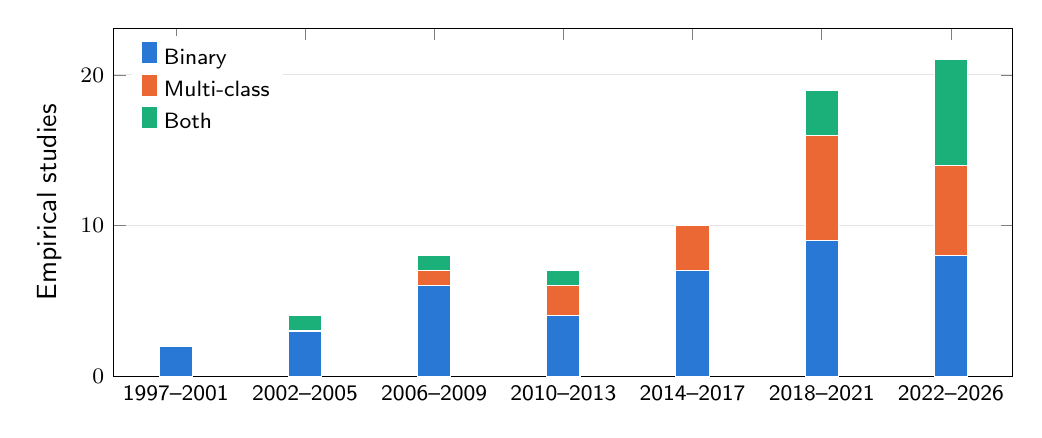
\begin{tikzpicture}
\begin{axis}[ybar stacked,width=13cm,height=6cm,bar width=12pt,ymin=0,xtick={0,...,6},xticklabels={{1997--2001},{2002--2005},{2006--2009},{2010--2013},{2014--2017},{2018--2021},{2022--2026}},
  ylabel={Empirical studies},enlarge x limits=0.08,tick label style={font=\footnotesize},legend cell align=left,legend style={font=\footnotesize,at={(0.02,0.98)},anchor=north west,draw=none},ymajorgrids,grid style={gray!20}]
\addplot[fill=sOne,draw=white] coordinates {(0,2) (1,3) (2,6) (3,4) (4,7) (5,9) (6,8)};
\addplot[fill=sTwo,draw=white] coordinates {(0,0) (1,0) (2,1) (3,2) (4,3) (5,7) (6,6)};
\addplot[fill=sThree,draw=white] coordinates {(0,0) (1,1) (2,1) (3,1) (4,0) (5,3) (6,7)};
\legend{{Binary},{Multi-class},{Both}}
\end{axis}
\end{tikzpicture}
\end{document}
